\documentclass[10pt,a4paper]{article}
\usepackage[margin=1.25in]{geometry}
\usepackage{fancyhdr} % fancy header
\pagestyle{fancy} % so fancy
\usepackage[round]{natbib} % bibliography
\usepackage{graphicx} % for importing graphics / figures
\usepackage{booktabs} % publication-worthy tables
\usepackage{multirow}
\usepackage{adjustbox} % makes tables fit nicely on the page


\lhead{Josh MEYER}
\rhead{Dissertation Prospectus}
\cfoot{} %% make empty to get rid of the page number %% \cfoot{Page \thepage}
\renewcommand{\footrulewidth}{0.4pt} %% this puts a fancy line at the footer


\begin{document}


\section{What I'm doing \& Why it's Extremely Cool}

I'm creating Neural Nets which better classify data from unseen conditions, without any explicit adaptation of model parameters or data transformations. In my dissertation, the neural nets of interest are acoustic models for automatic speech recognition, and the unseen data conditions are (1) \texttt{new noise}, (2) a \texttt{new speaker}, or (3) a \texttt{new language}. For each of these three cases, I have two conditions of data. I train the model on one data condition, and then test the on other.

\begin{enumerate}
  
\item For the \texttt{Noise} condition, I train on clean audio and test on noisy audio.
\item For the \texttt{Speaker} condition, I train on a set of speakers, and I test on an unseen speaker.
\item For the \texttt{Language} condition, I train on (mostly) English, and I test exclusively on Kyrgyz. I must include \textit{some} Kyrgyz in training because the DNN+HMM pipeline requires the testing phonemes defined in the model.  
  
\end{enumerate}
    
My approach is extremely cool because it doesn't require tons of data, it is not specific to some dataset, and it can be used to train any Neural Net (not just for speech recognition).

In the past people have dealt with new data by (1) adapting an existing model to the new data, or (2) normalizing the new data to look more like the old training data. More recently, Multi-Task Learning (MTL) has been found to produce models which are better at handling new data, because these models inherently learn more robust features which generalize to unseen domains. 

MTL training for neural nets works by training a set of hidden layers to perform multiple tasks (multiple output layers). Here is an example of MTL architecture for an acoustic model from Heigold 2013.

\begin{center}
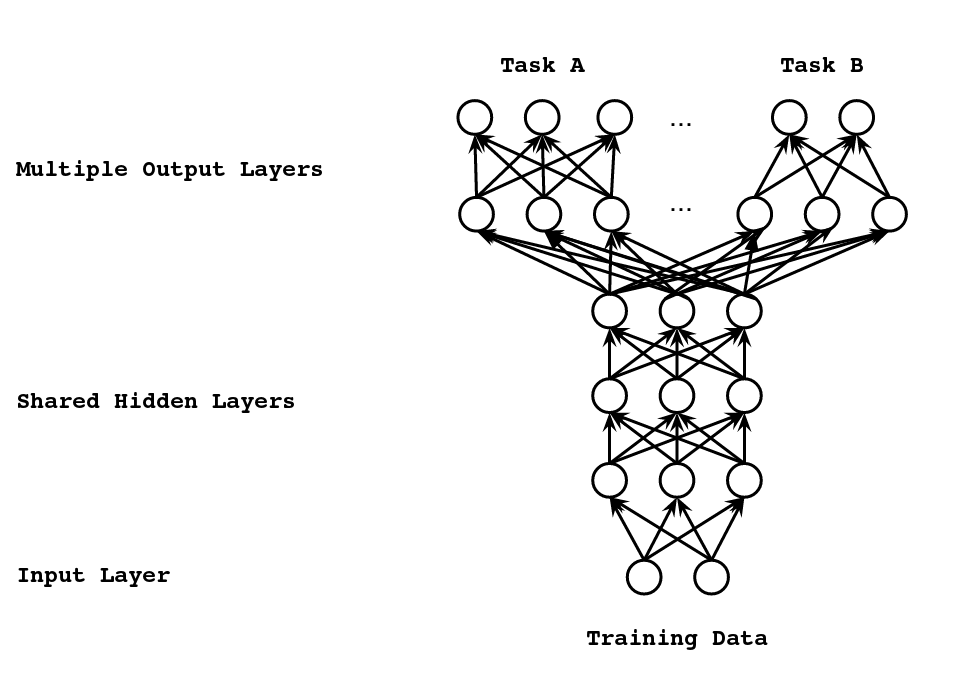
\includegraphics[width=.85\textwidth,keepaspectratio]{figs/heigold-2013-dnn-c.png}
\end{center}

This is the same architecture that will be used in my dissertation, but obviously I will have more layers and more nodes per layer. The number of input nodes on my neural nets corresponds to the dimensionality of audio features, and the number of nodes on each output layer corresponds to the number of phonemes (i.e. monophones or triphones) I've defined for the language.

In this dissertation (following the MTL tradition), each output softmax layer will be referred to as a \texttt{Task}.
\section{Overview of Speech Recognition}

This section contains an overview of the training and testing procedures for standard automatic speech recognition (ASR) pipelines. The overview will provide the reader with a technical grounding in ASR, so that the rest of the dissertation will have some point of reference. 


\begin{itemize}

\item \textbf{Gaussians + HMMs}
  
\item \textbf{Neural Nets + HMMs}
  
\item \textbf{end-to-end Neural Nets}

\end{itemize}


\section{Background Literature}

Here I will cover the literature relevant to working with small (or completely new) datasets. There are two main approaches, (1) adapt a model from one training dataset to a new, smaller dataset; (2) create a model that is robust enough to handle data from multiple domains. 

\begin{itemize}

\item \textbf{Model Adaptation: (e.g. Speaker; Language)}

      %% 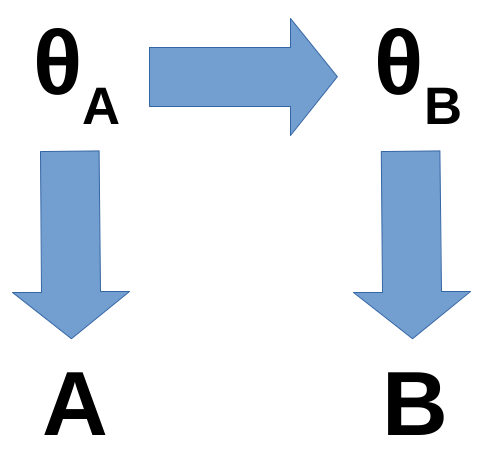
\includegraphics[width=.2\textwidth,keepaspectratio]{figs/transfer.png}
    
  
\item \textbf{Model Robustness: (e.g. Noise; Channel)}

    %% 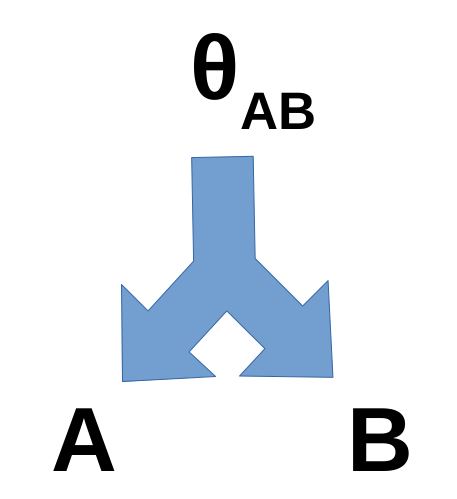
\includegraphics[width=.2\textwidth,keepaspectratio]{figs/robustness.png}
  
\end{itemize}




\section{Experiments}

This section contains the main contributions of the dissertation research.

This dissertation investigates training methods for acoustic modeling in the Neural Net + HMM ASR pipeline.

I aim to produce acoustic models which perform better (i.e. lower Word Error Rates) on datasets which are not similar the original training dataset.

I investiage the effectiveness of different \texttt{Tasks} (eg. linguistic \texttt{Tasks} vs machine learning \texttt{Tasks}) in a Multi-task Learning framework.


\subsection{Data}

I am creating acoustic models which generalize well to new data. To measure how well the models generalize, I use a set of speech corpora which exhibit some interesting differences between training and testing data. These differences between corpora exemplify the typical challenges faced in speech recognition generalization.

The training and testing data will differ in either (1) the recording \texttt{noise} conditions, (2) who the \texttt{speaker} is, or (3) what \texttt{language} the speaker is using. The following table shows which data sets are used for each audio condition.


\begin{table}[htbp]
  \centering
  \begin{adjustbox}{width=.75\textwidth}
    \begin{tabular}{clcc}
      \toprule
      && \multicolumn{2}{c}{\textsc{Corpus}}\\
      && \textbf{Train} & \textbf{Test}\\
      \midrule
      \multirow{3}{*}{\textsc{Audio Condition}} &\textbf{Noise} & TIDIGITS & Aurora 5 \\
      &\textbf{Speaker} & LibriSpeech-A & LibriSpeech-B \\
      &\textbf{Language} & LibriSpeech & Kyrgyz Audiobook \\
      \bottomrule
    \end{tabular}
    \label{table:data}
  \end{adjustbox}
  
  \caption{Speech Corpora}
  
\end{table}


\subsection{Model Training Procedure}

This dissertation investigates the creation of new tasks for MTL, either using (1) linguist-expert knowledge, (2) ASR Engineer-expert knowledge, or (3) general Machine Learning knowledge.

The former two knowledge sources are useful for buidling acoustic models, but not much else. On the other hand, the final knowledge source (general machine learning concepts) can be applied to \textit{any} classification problem.

The three knowledge sources will be abbreviated as such:
  
\begin{itemize}
\item  (\textsc{LING}) \textbf{Linguistic Knowledge} 
\item (\textsc{ASR}) \textbf{Traditional Speech Recognition Pipeline}
\item (\textsc{ML}) \textbf{General Machine Learning}
\end{itemize}


Each of these categories contains a wealth of ideas, but I will consolidate each into three experiments. With three experiments for each knowledge source, my dissertation will contain nine (9) experimental conditions (for each audio condition).

Specifically, I will use the following concepts to create new tasks to be used in MTL training:

\begin{table}[htbp]
  \centering
  \begin{adjustbox}{width=.75\textwidth}
    \begin{tabular}{cccc}
      \toprule
      & \multicolumn{3}{c}{\textsc{Knowledge Source}}\\
      & \textbf{LING} & \textbf{ASR} & \textbf{ML}\\
      \midrule
      \multirow{3}{*}{\textsc{Experiments}} & voicing & monophones &  k-means \\
      & place & $1/2$ triphones & random forests  \\
      & manner & $3/4$ triphones &  bootstrapped resamples  \\
      \bottomrule
    \end{tabular}
    \label{table:data}
  \end{adjustbox}
  
  \caption{Experimental Setup}
  
\end{table}


Each of these tasks will be added to a Baseline model. More specifically, the Baseline model will be a Neural Net with a single output layer (Task A), and the tasks above will be added as a second task (Task B). You can think of the tasks as simply a new set of labels for the existing data set. For example, when the \textsc{Ling} task of \textsc{voicing} is used, any audio segment labeled \texttt{[b]} will be assigned the new label \texttt{voiced}.

When these experiments will be applied to each of the three audio conditions, we get the following 30 experiments:

\begin{table}[htbp]
  \centering
  \begin{adjustbox}{width=.95\textwidth}
    \begin{tabular}{ccclc}
      \toprule
      \textbf{Data Condition} & \textbf{Train Data} & \textbf{Test Data} & \textbf{MTL Training Tasks} & \textbf{Num. Exps} \\
      \midrule
      \multirow{4}{*}{\textsc{Noise}} & \multirow{4}{*}{\textsc{TIDIGITS}} & \multirow{4}{*}{\textsc{Aurora 5}} & Basline & 1\\
      & & & Baseline + LING & 3   \\
      & & & Baseline + ASR  & 3  \\
      & & & Baseline + ML   & 3  \\
      \midrule
      \multirow{4}{*}{\textsc{Speaker}} & \multirow{4}{*}{\textsc{LibriSpeech-A}} & \multirow{4}{*}{\textsc{LibriSpeech-B}} & Baseline & 1 \\
      & & & Baseline + LING & 3  \\
      & & & Baseline + ASR  & 3  \\
      & & & Baseline + ML   & 3  \\     \midrule
      \multirow{4}{*}{\textsc{Language}} & & \multirow{4}{*}{\textsc{Kyrgyz-B}} & Baseline & 1\\
      & \textsc{LibriSpeech +} & & Baseline + LING  & 3 \\
      &  \textsc{Kyrgyz-A} & & Baseline + ASR   & 3 \\
      & & & Baseline + ML & 3 \\
      \midrule
      &&&& 30\\
      \bottomrule\\
    \end{tabular}
    \label{table:data}
  \end{adjustbox}
  
  \caption{Experimental Setup}
  
\end{table}


\newpage

\subsection{Task Creation Specifics}


\begin{enumerate}

\item \textbf{Baseline}

All the following architectures will be compared to the performance of the following baseline.

To account for any advantage mutliple output layers may bring about, the baseline also contains two output layers, where the \texttt{Tasks} are identical. In this way, random initializations in the weights and biases for each \texttt{Task} are accounted for.

During testing, \textit{only one} of the \texttt{Tasks} is used. The additional \texttt{Tasks} are dropped and the \texttt{Baseline Triphones} are used in decoding. This highlights the purpose of the extra \texttt{Tasks}: to force the learning of robust representations in the hidden layers during training. The \texttt{Tasks} may in fact not be the best option for final classification; they serve as ``training wheels'' which are then removed once the net is ready. 

\begin{figure}[!htb]
  \centering
\minipage{0.66\textwidth}
  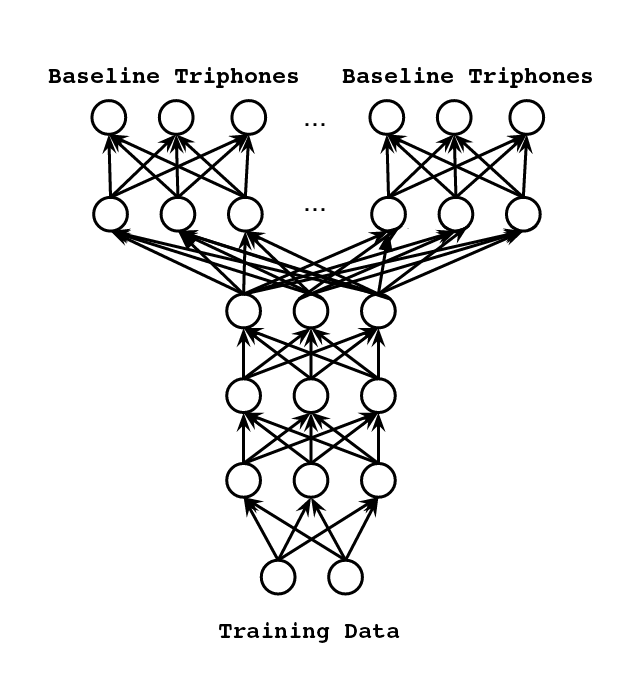
\includegraphics[width=\linewidth]{figs/mtl-arch-baseline.png}
  \caption{\texttt{Baseline}}
\endminipage\hfill
\end{figure}



\newpage
\item \textbf{LING}

  All of the linguistic knowledge tasks view the phoneme as a bundle of features.

  Using standard features from articulatory phonetics (voicing, place, and manner), the following tasks generate labels for each data point by collapsing the given phoneme labels along one of these three dimensions.

  All information from one dimension is removed from the labeled data. This forces the classifier to rely on audio signal features which do not relate to that dimension. The DNN must project the input data into a new space for classification, using only information from the other two dimensions. 

  
  \begin{enumerate}
  \item \textsc{voicing}

    Voicing information is removed from the data labels.

  \item \textsc{place}

    All place information is removed from the data labels.
    
  \item \textsc{manner}
    
    All manner information is removed from the data labels.
    
  \end{enumerate}


\begin{figure}[!htb]
\minipage{0.32\textwidth}
  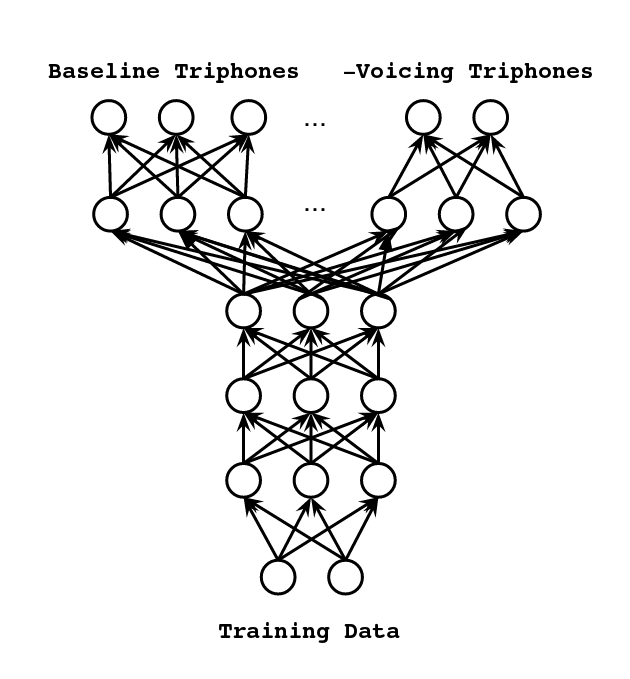
\includegraphics[width=\linewidth]{figs/mtl-arch-voicing.png}
  \caption{\texttt{-Voicing}}
\endminipage\hfill
\minipage{0.32\textwidth}
  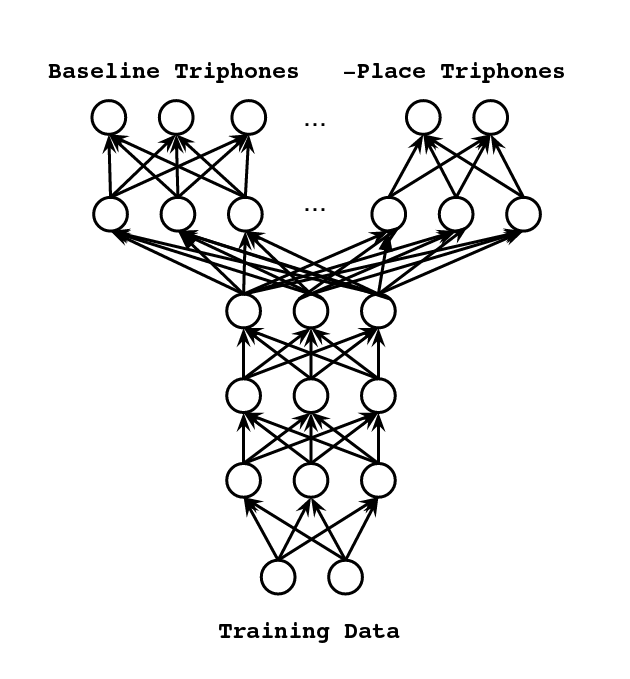
\includegraphics[width=\linewidth]{figs/mtl-arch-place.png}
  \caption{\texttt{-Place}}
\endminipage\hfill
\minipage{0.32\textwidth}%
  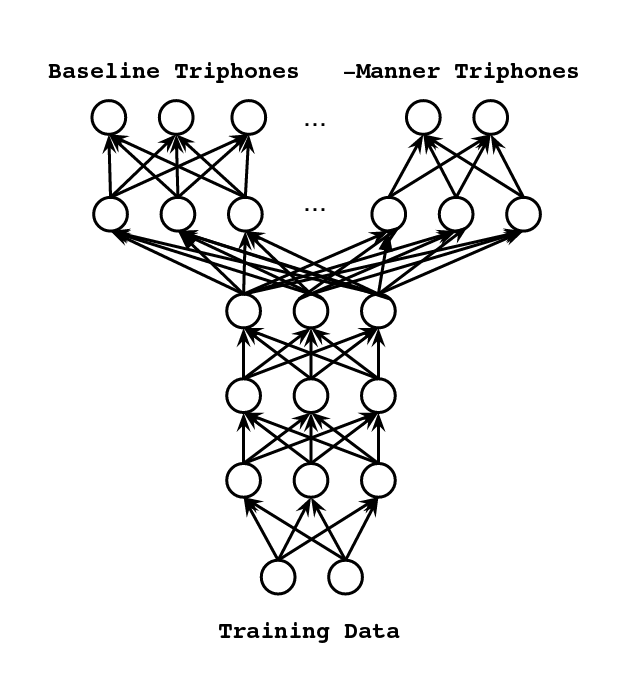
\includegraphics[width=\linewidth]{figs/mtl-arch-manner.png}
  \caption{\texttt{-Manner}}
\endminipage
\end{figure}



\newpage

\item \textbf{ASR}

  All the following tasks relate to the structure of the phonetic decision tree used in the traditional ASR pipeline to cluster context-dependent triphones. In GMM training the leaves of the decision tree are then assigned their own Gaussians, and in DNN training the same leaves are used as labels during training via backprop.

  The main intuition behind these experiments is that in using the decision tree labels as targets for the DNN classifier, we are performing model transfer. The decision tree and it's associated Gaussians perform classification, and we are merely training a DNN to perform that same task. So, the decision tree can be thought of as a single task for the DNN to learn.

  However, the DNN only sees the leaves of the decision tree. It doesn't see any of the branches, or any of its wonderful linguistic structure. So, in order to force the DNN to learn the information hidden in the decision tree, the following tasks are like cross-sections of the tree, slicing it from leaves up. The DNN then has to learn how to read these cross-sections, and how to map data onto each layer.

  If we slice the tree at the roots, we have the \textsc{monophones}. If we slice down half-way (\textsc{1/2 triphones}), we have more contextual information than monophones but less than full triphones. If go a little farther down (\textsc{3/4 triphones}), we get even more context, but less general information about the original phoneme.
  
  \begin{enumerate}
  \item monophones

    When we chop the tree at the roots.
    
  \item 1/2 triphones

    Chop the tree half-way down.
    
  \item 3/4 triphones

    Chopping a little further.
    
  \end{enumerate}


  

\begin{figure}[!htb]
\minipage{0.32\textwidth}
  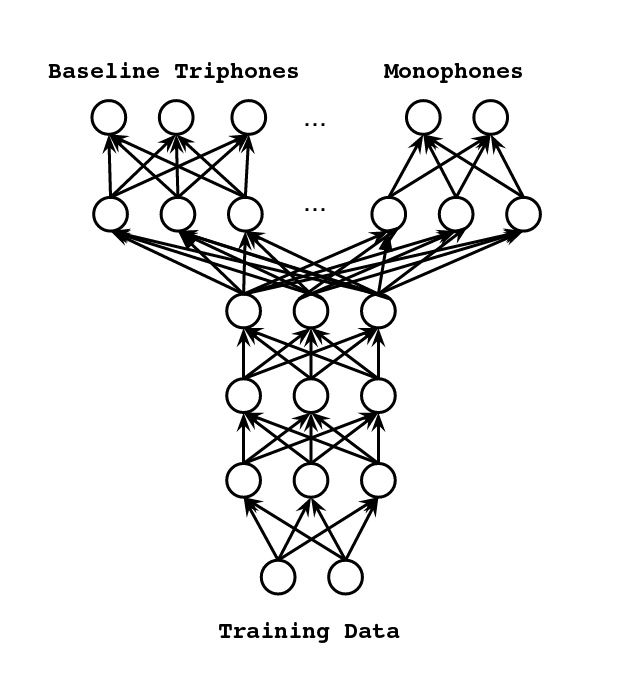
\includegraphics[width=\linewidth]{figs/mtl-arch-mono.png}
  \caption{\texttt{Monophones}}
\endminipage\hfill
\minipage{0.32\textwidth}
  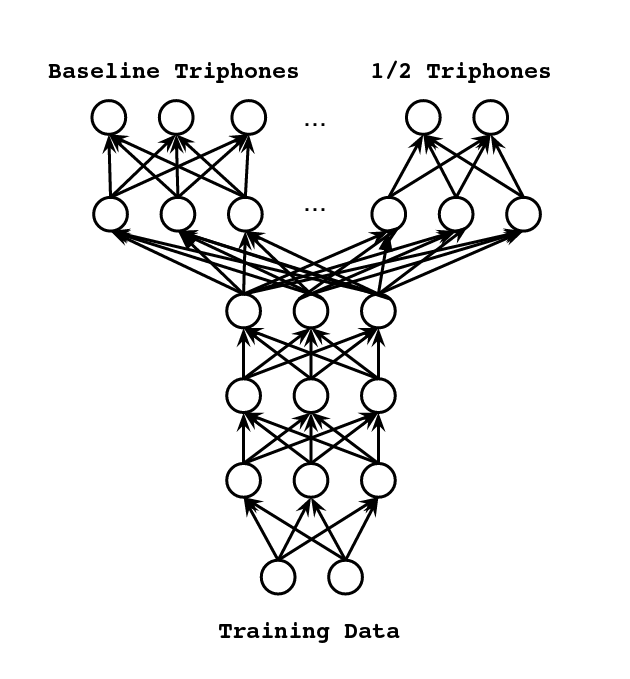
\includegraphics[width=\linewidth]{figs/mtl-arch-halfTri.png}
  \caption{\texttt{1/2 Triphones}}
\endminipage\hfill
\minipage{0.32\textwidth}%
  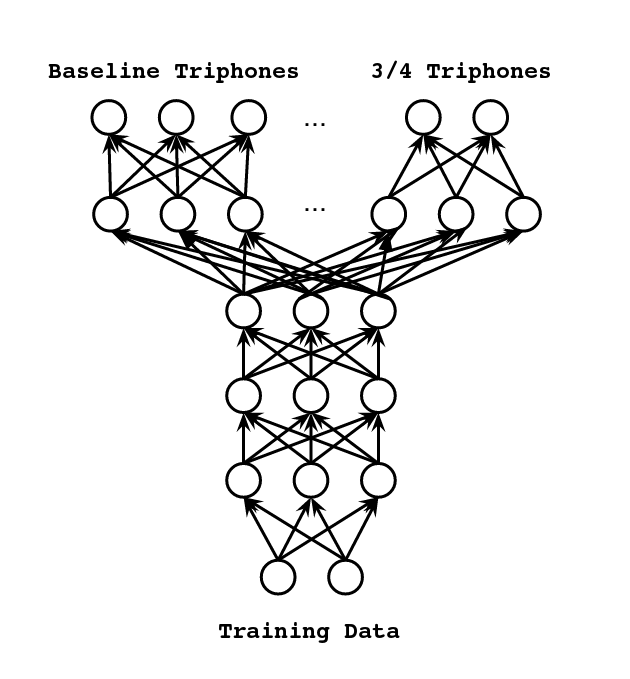
\includegraphics[width=\linewidth]{figs/mtl-arch-3QuarterTri.png}
  \caption{\texttt{3/4 Triphones}}
\endminipage
\end{figure}


\newpage

\item \textbf{ML}

  The following tasks do not make use of any linguistic knowledge or any part of the ASR pipeline. The only things needed to perform these tasks is labeled data.

  The two approaches above use linguistics or the ASR pipeline to force a DNN to learn structure about the data, because that information is useful for classification.

  We typically do not have this kind of \textit{a priori} information about the datasets we use in Machine Learning. Therefore, an interesting problem is how to learn this structure in a data set when we don't have access to that expert knowledge.

  The following tasks force the DNN to learn structure in the data without any knowledge about that structure. In order to do so, I make the assumption that the data does in fact have heirarchical relations. That is, I assume the \texttt{(data,label)} pairs were generated by something like a phonetic decision tree, and I try to recover the structure of that tree.
  
  \begin{enumerate}
  \item k-means

    Standard k-means on the data, with the caveat that labels cannot be split across clusters. A first round of clustering is performed, and then all data from the same original label are shifted to the cluster with the most data points from that label. Then, centroids are recalculated, and data is re-clustered. This adapated k-means should find related data points in the same clusters. If k-means is working, we would expect to be able to recover phonemes (monophones) from the labeled triphone data.
    
  \item random forest

    In another attempt to cluster triphones along phonetic categories, the random forest procedure works as follows: (1) take a random subset of the labels, (2) train a random forest with all data points associated with those labels, (3) re-classify all the rest of the data with the new random forest. In this way, we will reduce the number of labels (eg. out of 2,000 triphone labels I choose 500), and classify unseen data as its closest seen data point.

  \item bootstrapped resamples

    In this approach, new labels are not generated at all. The separate tasks for the DNN are just different samples of the data.

    Some sub-samples may exhibit a more useful decision plane than others, and if we randomly subsample for multiple tasks, the different decision planes will all have something in common. The individual peculiarities of one sub-sample will have to be ignored for the DNN to perform well on all tasks.
    
  \end{enumerate}

\begin{figure}[!htb]
\minipage{0.32\textwidth}
  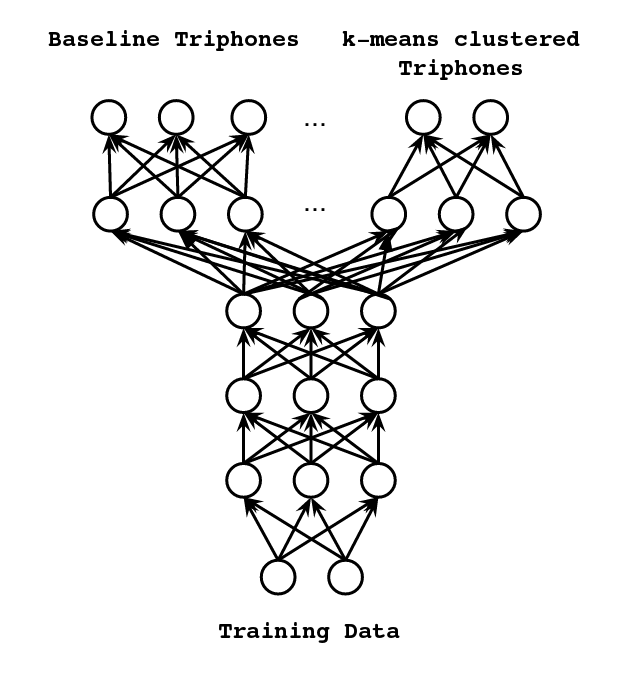
\includegraphics[width=\linewidth]{figs/mtl-arch-kMeans.png}
  \caption{\texttt{k-means}}
\endminipage\hfill
\minipage{0.32\textwidth}
  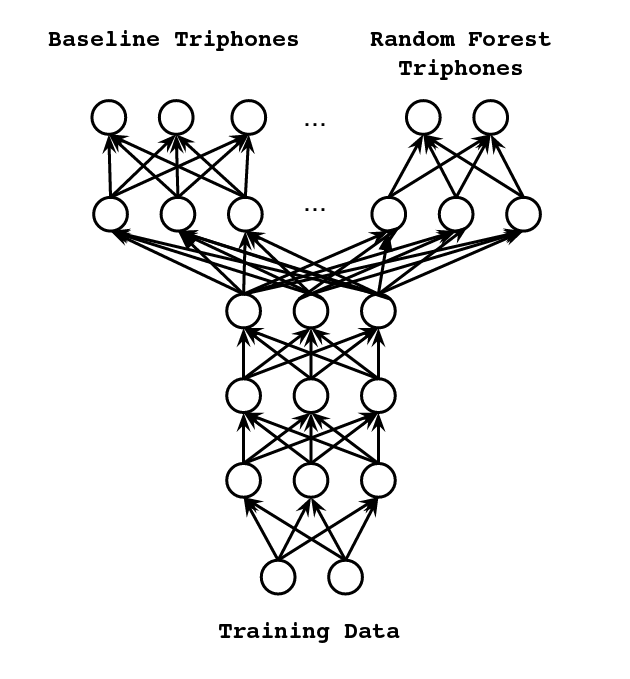
\includegraphics[width=\linewidth]{figs/mtl-arch-forest.png}
  \caption{\texttt{1/2 Triphones}}
\endminipage\hfill
\minipage{0.32\textwidth}%
  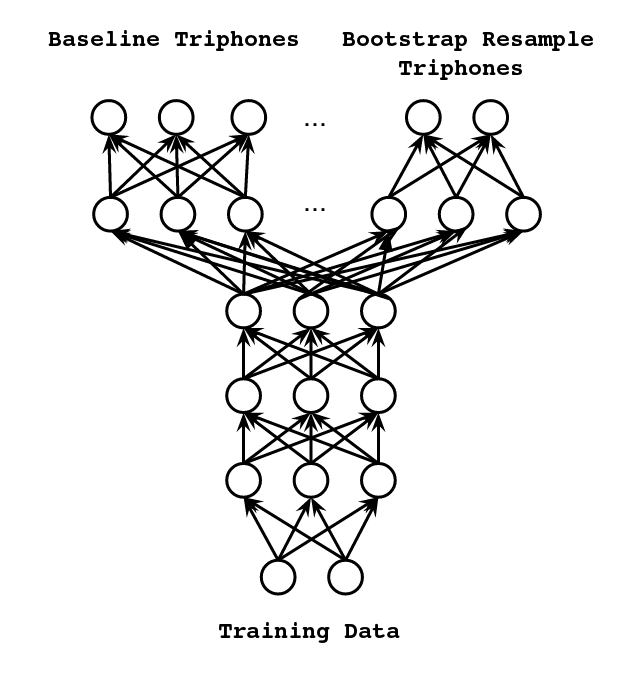
\includegraphics[width=\linewidth]{figs/mtl-arch-resampled.png}
  \caption{\texttt{3/4 Triphones}}
\endminipage
\end{figure}





\end{enumerate}








\end{document}



 
